% Latex template
\documentclass[
	10pt, % Default font size, values between 10pt-12pt are allowed
	%letterpaper, % Uncomment for US letter paper size
	spanish, % Uncomment for Spanish
]{fphw}

% Template-specific packages
\usepackage[utf8]{inputenc} % Required for inputting international characters
\usepackage[T1]{fontenc} % Output font encoding for international characters
\usepackage{mathpazo} % Use the Palatino font
\usepackage{graphicx} % Required for including images
\usepackage{booktabs} % Required for better horizontal rules in tables

\usepackage{listings} % Required for insertion of code

\usepackage{enumerate} % To modify the enumerate environment
\usepackage{listings}
\usepackage{amsmath}

% titles 

\title{Práctica 2: codificación de canle}

\author{Miguel Blanco Godón}

\date{2 de maio do 2021}

\institute{Universidade da Coruña \\ Facultade de Informática} 

\class{Software de comunicacións (Enxeñaría de computadores)}

\professor{Óscar Fresnedo Arias} 

% actual document

\begin{document}

\maketitle 

\section*{Introdución}
O obxectivo desta práctica é ampliar o estudo dos sistemas de comunicación á condificación de canle. O método de estudo será a simulación en Matlab. En concreto, estudaranse os códigos de repetición factor 3 e 5, os códigos de Hamming (7,4) e tres códigos convolucionais distintos.
\section*{Arquitectura do sistema}
O sistema extende a práctica anterior, engadindo 2 novos módulos: un codificador antes do modulador e un decodificador despois do demodulador. A canle seguirá a ser unha canle AWGN, pero cuxa varianza será modificada cando se transmitan datos codificados para garantir unha correcta comparación coas transmisións non codificadas.
A continuación exporase a arquitectura dos novos módulos e os cambios nos antigos.
\subsection*{Codificador}
Encárgase de convirtir os bits fonte en palabras código segundo o código especificado. 
O codificador está dentro do módulo de transmisión do sistema, e delega o traballo de codificación nun encoder/decoder específico no caso de usar códigos de repetición ou Hamming, e por implementación directa a partir das funcións do \textit{Communications toolbox} de Matlab no caso dos códigos convolucionais.
\subsection*{Decodificador}
Forma parte do receptor, solidario ao demodulador. O seu traballo é a recuperación e corrección de erros de transmisión.
Igual cao codificador, sitúase dentro do módulo de transmisión e tamén delega a codificación en función da operación solicitada. 
\subsection*{Canle AWGN}
A canle foi modificada para aumentar a varianza do ruído cando se transmiten datos codificados, no mesmo factor que aumenta o número de bits de redundancia. Isto faise para permitir unha comparación válida, posto que os bits de redundancia da codificación son eliminados na decodificación, polo que de non aumentar o ruído de xeito proporcional a esta redundancia teriamos menos erros (ficticiamente) ao eliminar parte dos bits recibidos.
\section*{Implementación}
Explicarase a o funcionamento dos encoders para cada tipo de código:
\subsection*{Códigos de repetición factor R} 
Está implementado no ficheiro "rept\_code.m". Consiste na repetición de cada bit da entrada R veces. Pódese implementar rápidamente mediante a replicación do vector de bits fonte e un reshape correspondente (de tal xeito que o vector resultante sexa a concatenación das columnas da matriz resultante da replicación). Para a decodificación, faise a operación de reshape inversa. Posteriormente súmase a matriz por columnas. Deste xeito, podemos decodificar corrixindo ata $\frac{R-1}{2}$ erros. Se para cada $i$, $\frac{1}{2} \sum_{i, j=0}^{j=R} recv[i,j] \leq \frac{R}{2}$, a sáida do codificador será 0, senón, 1.
\subsection*{Códigos de Hamming}
Está implementado no ficheiro "hamming\_code.m". A implementación funciona para calquer código de Hamming con $n = 2^{l}-1$, sempre que $n \geq 7$.
O módulo está partido en 4:
\begin{itemize}
\item \textbf{Xeración de $H$}:
directamente cunha conversión a binario en formato MSB de $0$ a $2^n-1$ dun vector 1:n.
\item \textbf{Xeración de $G$}:
calcúlase a partir da matriz de control de paridade $H$. Os valores de $n$ e $l$ correspóndense co número de columnas e filas da matriz $H$.
A partires disto, definin uns vectores de índices para a permuta das filas e das columnas para obter G. Entón, o vector de índices de permuta 
$\vec{a} = a_{k} = 2^k$ entre $k = 1$ e $2^k \leq n$. As columnas correspondentes con estes índices son permutadas coas columnas cuxos índices se 
gardan en $\vec{b} = b_k = n+1-(l-k)$.
A continuación realízase a permutación $H_{i} \Longleftrightarrow H_{j}$ onde $i \in a_k$ e $j \in b_k$.
Ademais, as columnas $c_k \notin \vec{a},\vec{b}$ desprázanse ás primeiras posicións de $H$, quedando co seguinte formato
\newline 
\newline 
$H = H(P^T | I_{lxl}) = $
\begin{pmatrix}
c_{00} & c_{01} & ... & c_{0(2l-1)} & b_{00} & ... & b_{0l} & a_{00} ... & a_{0l} \\
c_{10} & c_{11} & ... & c_{1(2l-1)} & b_{10} & ... & b_{1l} & a_{10} ... & a_{1l} \\ 
.&.&...&.&.&...&.&...&. \\
.&.&...&.&.&...&.&...&. \\
.&.&...&.&.&...&.&...&. \\
c_{(n-l)0} & c_{(n-l)1} & ... & c_{(n-l)(2l-1)} & b_{(n-l)0} & ... & b_{(n-l)l} & a_{(n-l)0} ... & a_{(n-l)l} 
\end{pmatrix}
\newline
\newline
\newline
Despois concaténase  as partes para formar $G' = G'(I_{(n-l)x(n-l)} | P)$. Por último, só restaría desfacer as permutas para obter a matriz $G$ tal que
$G H^T = 0$.
\item \textbf{Codificación}:
para a codificación faise un reshape para que entren os bits $M$ en filas de $n-l$ columnas, faise o produto $M G$ e desfaise o reshape para volver a obter un vector fila.
\item \textbf{Decodificación}:
debemos facer un reshape dos bits de entrada $R$ para que sexan filas de $n$ columnas. Faise a multiplicación $S = RH^T$ para obter o síndrome, $S$.
Ese síndrome ten en cada fila, en binario (MSB de $0$ a $2^n -1$) a posición por fila de R onde houbo un erro sempre e cando $S_k \neq 0$. Confecciónase un vector de índices (para saber qué filas hai que cambiar) faise un \textit{bit flip} para corrixir os fallos. Por último, restaría quitar as columnas que son externas aos bits fonte, que coinciden coas do vector $\vec{a}$ do apartado anterior. Unha vez feito iso, cun reshape podemos volver a obter os bit fonte.
\end{itemize}
\subsection*{Códigos convolucionais}
Están implementados directamente no módulo "transmit.m", debido a que se usan funcións da librería de comunicacións de Matlab. A implementación da codificación faise en dous pasos: a creación do diagrama de trellis, e o uso da función "convenc". Para a decodificación, úsase o algoritmo de Viterbi. Agora exporei os parámetros dos códigos convolucionais usados (a partir dos diagramas):
\begin{itemize}
\item \textbf{Conv I}:
son 3 rexistros, polo que o rate do código é $\frac{1}{3}$. A saída sistema é, en octal [7 5 6].
\item \textbf{Conv II}:
son 3 rexistros tamén, polo que o rate do código é $\frac{1}{3}$. A saída do sistema é, en octal [3 5 6].
\item \textbf{Conv III}:
son 4 rexistros, polo que o rate do código é $\frac{1}{4}$. A saída do sistema é, en octal [17 13 15 11]. Correspóndese cun código cunha distancia libre de 12.
Para o deseño do código tiven en conta dous parámetros: a distancia libre ($d_H$) e \textit{constraint length} ($m$). Tendo en conta que necesitaba un código que me dera máis ganancia de codificación,
tiña que obter unha relación entre $d_H$ e $m$ tal que fose maior ca do código «Conv I», para paliar os efectos da ganancia de ruido asociada na simulación. Despois de probar varios códigos, decanteime polo definido anteriormente,
xa que cumpría os requisitos, $\frac{12}{4} > \frac{7}{3}$.
\end{itemize}
\section*{Resultados}
En todas as probas os esquemas de modulación utilizaron mapeado de Gray.
\subsection*{Repetición}
Os resultados foron malos debido ao axuste no ruído xerado pola canle. Como a varianza do mesmo se multiplica por $\frac{n}{k}$, os códigos de menor rate veranse perxudicados. Vense perxudicados xa que temos que ter en conta o aumento da enerxía de bit, xa que por cada bit de datos, debemos transmitir $R$ veces máis. Deste xeito, para o código con $R = 3$, teriamos o triplo de enerxía por bit, e para o caso de $R = 5$, teriamos 5 veces máis.
Isto leva a un aumento directamente proporcional e na mesma cantidade da varianza do ruido, o que fai que se produzan moitos erros de bit, e que fai que o decodificador produza moitos erros, lastrando o rendemento da transmisión.
Entón temos un código moi simple de implementar, que se podería facer en hardware moi rápido e de xeito sinxelo, pero cunha ganancia de codificación nula ou negativa.
\begin{figure}[htb]
\centering
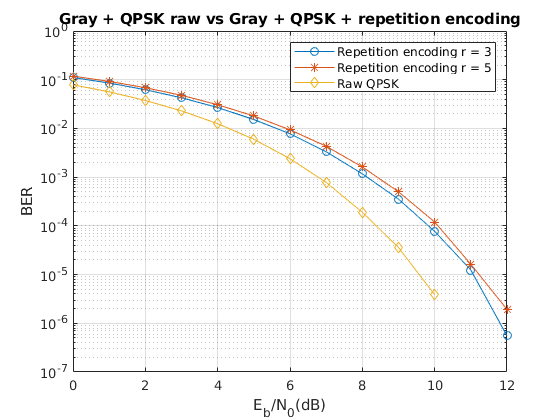
\includegraphics{repetition.png}
\caption{Resultados para os códigos de repetición}
\end{figure}
\subsection*{Hamming}
Os resultados varían en función do valor de $E_b N_0$. Para $E_b N_0 < 6 \quad dB$, temos máis erros ca a transmisión modulada sen codificación. No caso contrario, mellora a capacidade de detección e corrección do código e obtemos
un menor número de erros de bit. Isto débese a dous factores. O primeiro, que a redundancia engadida ao código fai que se xere moito ruído (debido ao axuste de varianza) e segundo, que un código de Hamming sempre vai corrixir 1 só erro, polo que en caso de haber múltiples erros na transmisión, decodificaremos mal. Por iso para valores pequenos de $E_b N_0$ onde a varianza é alta, temos unha mala resposta do esquema de codificación, mentres que cando temos valores máis favorables obtemos unha ganancia de codificación positiva, cercana a $ 5 \cdot 10^{-1} \quad dB/E_bN_0$ con respecto aos valores sen codificar.
Con respecto á modulación utilizada, vemos un pequeno aumento de rendemento cando se combina con 16-QAM, pero con todo as dúas ganancias son bastante semellantes. Creo que o motivo é que os códigos de Hamming sempre corrixen 1 só erro, polo que a ganancia máxima de codificación que imos ter tenderá a ser constante e próxima ao rendemento da transmisión non codificada.
\begin{figure}[htb]
\centering
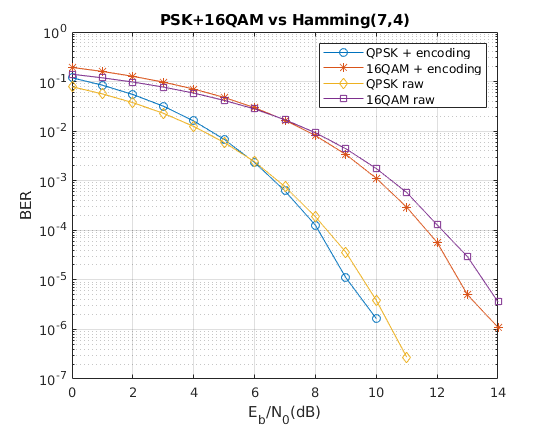
\includegraphics{hamming.png}
\caption{Resultados para o código de Hamming(7,4)}
\end{figure}
\subsection*{Códigos convolucionais}
Neste caso hai moita disparidade en función do código escollido. Para o primeiro e o terceiro código, ocorre o mesmo ca co código de Hamming: para valores pequenos de $E_bN_0$, temos unha ganancia de codificación negativa, mentres que para valores altos, unha ganancia de codificación alta, notablemente superior á obtida con códigos de Hamming. Esta ganancia de codificación tamén aumenta ao pasar de QPSK a 16-QAM. 
Este aumento é maior ca o obtido co código de Hamming, xa que un código convolucional pode corrixir $\lfloor \frac{d_{min} - 1}{2} \rfloor$ erros, polo que no caso do primeiro código teríamos unha capacidade correctora
de 3 erros, mentres ca o terceiro pode corrixir ata 5.
\newline
O segundo código é un caso aparte. Se intentamos calcular a súa distancia libre (\textit{distspec}), observamos que é un \textit{código catastrófico}. Un código catastrófico é un código convolucional que é propenso á propagación
de erros catastróficos, é dicir, que permite que se dea a situación na que un número finito de erros na canle provoque un número infinito de erros no decodificador. 
Para comprender isto é útil observar a táboa de estados do código:
\begin{center}
\begin{tabular}{ |c|c|c|c| }
\hline
\textbf{ENTRADA} & \textbf{ESTADO ACTUAL} & \textbf{ESTADO SEGUINTE} & \textbf{SAÍDA} \\
\hline
0 & 00 & 00 & 000 \\
\hline
1 & 00 & 10 & 011 \\
\hline
0 & 01 & 00 & 110 \\
\hline
1 & 01 & 10 & 101 \\
\hline
0 & 10 & 01 & 101 \\
\hline
1 & 10 & 11 & 110 \\
\hline
0 & 11 & 01 & 011 \\
\hline
1 & 11 & 11 & 000 \\
\hline
\end{tabular}
\end{center}
Aqui podemos ver o fallo do código: para unha secuencia de todos ceros, a saída do codificador sería todo ceros. Se metemos todo uns, a saída do codificador sería 0111100000000... o que nos indica que malia que nós metamos dúas entradas cun número infinito de posicións distintas, o codificador saca dúas secuencias de saída que só difiren nun número finito de bits. Deste xeito, na decodificación, un número finito de erros na transmisión podería provocar un número infinito de erros na decodificación. Por iso se trata dun código catastrófico, como reflexan os resultados da simulación.
\begin{figure}[htb]
\centering
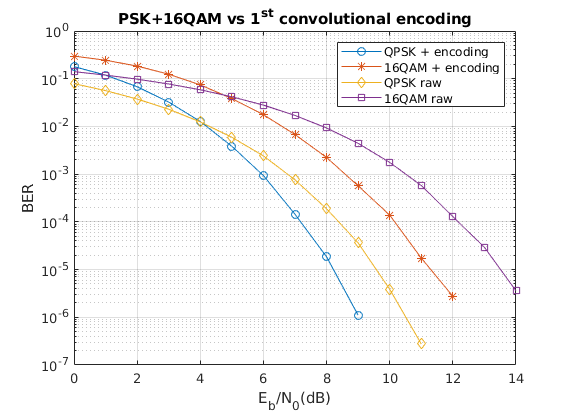
\includegraphics{fst.png}
\caption{Resultados para o código convolucional G = [7 5]}
\end{figure}
\begin{figure}[htb]
\centering
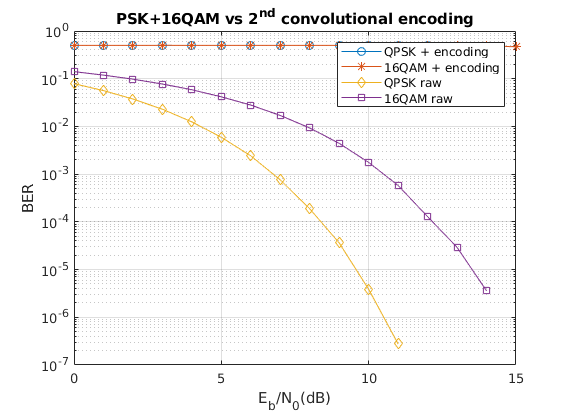
\includegraphics{snd.png}
\caption{Resultados para o código convolucional catastrófico}
\end{figure}
\begin{figure}[htb]
\centering
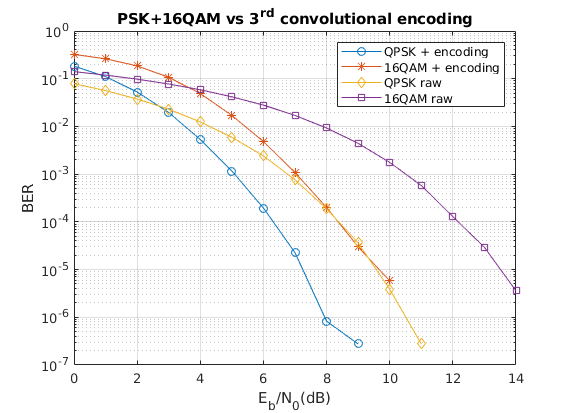
\includegraphics{third.png}
\caption{Resultados para o código convolucional G = [17 13 15 11]}
\end{figure}
\section*{Conclusións}
Ante a vista dos resultados hai dúas cousas claras: por unha banda, hai un conxunto de códigos desaconsellables en tódolos casos (polo menos nesta forma), e pola outra temos un conxunto de códigos útiles en determinadas circunstancias.
No primeiro grupo entrarían os códigos de repetición e os códigos catastróficos. Estes últimos son inútiles polas razóns anteriormente mencionadas. Os códigos de repetición empeoran os resultados debido ao baixo rate que teñen, sendo mellores canto maior é este último (menor $R$). Con todo, este grupo podería ser útil en caso de mesturalo con algún outro tipo de codificación como ocorre nos códigos concatenados e algúns códigos turbo, materia que sae fóra do estudo.
Por outra banda, temos os códigos «válidos», que son os que deron unha ganancia de codificación positiva con respecto aos datos sóamente modulados (Hamming e Conv I, III).
O feito de que estes esquemas de transmisión codificación + modulación só sexan beneficiosos a partires dun valor de $E_bN_0$ concreto e dependente do caso, lévame a pensar que:
\begin{itemize}
\item os tipos de codificación fonte estudados só se deberían usar despois de que unha prospección da canle nos dera uns valores de SNR aceptables.
\item en caso de manter a maior velocidade de transmisión deberíamos utilizar códigos de Hamming, posto que son os de menor rate, polo cal teñen menos redundancia e máis velocidade efectiva.
\item onde realmente é beneficiosa a codificación é utilizala conxuntamente con modulacións de un número de niveis elevados, como se pode ver co código convolucional 3.
Isto é precisamente porque nestes casos conséguese unha reducción dos erros/bit moito maior ca en esquemas de menos niveis, e ademais permítenos facelo sen reducir moito a velocidade de transmisión.
A velocidade de transmisión poderíase manter se temos unha modulación de varios niveis, por exemplo, 16-QAM ou superiores, nas cales transmitimos 4 ou maís bits/símbolo. 
Como se veu na práctica anterior estas modulacións son particularmente efectivas para canles con pouco ruido nas cales nos dá unha tasa de erros aceptable. 
Engadir nestes casos unha codificación como a convolucional implicaría que sen perder demasiada velocidade de transmisión, poderíamos utilizar 16-QAM coa mesma fiabilidade ca unha QPSK. 
A velocidade non se vería moi perxudicada xa que estamos doblando o número de bits por símbolo, aínda que aumentemos a redundancia. Polo que o importante sería ter un bo balance entre estos parámetros.
\end{itemize}

\end{document}
